%%%%%%%%%%%%%%%%%%%%%%%%%%%%%%%%%%%%%%%%%%%%%%
% Title: Quick Start Guide to LibreCAD       %
% Author: Jasleen Kaur                       %
% Email: jasleen.7956@gmail.com              %
%%%%%%%%%%%%%%%%%%%%%%%%%%%%%%%%%%%%%%%%%%%%%%

\documentclass[titlepage]{article}
\usepackage{graphicx}
\usepackage{fancyhdr}
\usepackage[margin=1.3in,footskip=0.25in]{geometry}

\title{Quick Start Guide to LibreCAD}
\author{Jasleen Kaur\\
Email: jasleen.7956@gmail.com\\
Blog: jasleen7956.wordpress.com}
}
\date{\today}
\pagestyle{fancyplain}
\fancyhf{}
\rhead{ \fancyplain{}{LibreCAD} }
\rfoot{ \fancyplain{}{\thepage} }
\lfoot{ \fancyplain{}{Jasleen Kaur: Quick Start Guide to LibreCAD} }
\renewcommand{\footrulewidth}{0.4pt}
\pdfpageheight =845pt   % to set height of paper


\begin{document}
\maketitle 
    \begin{abstract}
    This Quick Start Guide will help to introduce you with LibreCAD. If you have
    no experience of CAD before, then its a right place to start. This tutorial will make you familiar with many CAD concepts and it will also tell you how to use various functions and commands in LibreCAD. You need to keep
   patience while reading and enjoy the tutorial.
       \begin{flushright}
       Jasleen Kaur
       \end{flushright}
    \end{abstract}
\tableofcontents
\newpage

%whole content
\section{\textbf{Basics of CAD}}
\vspace{5 mm}  %to enter vertical space
\subsection*{Entities}
Entities are graphical objects in a CAD system. Typical entities which are supported by most CAD systems are: points, lines and circular and elliptical arcs. More complex and CAD specific entities include polylines, texts, dimensioning, hatches and splines.
\subsection*{Layers}
A basic concept in computer aided drafting is the use of layers to organize a drawing. Every entity in a drawing is on exactly one layer and a layer can contain lots of entities. Typically entities with a common 'function' or common attributes are put on the same layer. E.g. you might want to put all axes in a drawing on a layer named `axes'. Layers can have their own attributes also (colour, line width, line style etc...). Each entity can have its own attributes or have its attributes defined by the layer it is placed on. In the latter case for example you can change the colour of all the entities on the ``axes'' layer by setting the colour (red for example) for the layer `axes'.
\subsection*{Blocks}
A Block is a group of entities. Blocks can be inserted into the same drawing more than once with different Attributes and at different locations and at a different scale and rotation angle . Such an instance of a block is usually called an Insert. Inserts have attributes just like entities and layers. An Entity that is part of an Insert can have its own attributes or share the attributes of the Insert. Once created, Inserts are still linked to the Block they instantiate. The power of inserts is, that you can modify the Block once and all Inserts will be updated accordingly.
\subsection*{Coordinate System}
In order to get the best out of LibreCAD it is wise to have a good understanding of the coordinate system and how coordinates work. Everything that you draw in LibreCAD will be exact and precise and will be placed there accurately based on the X,Y coordinate system.
The absolute origin or Zero point in your drawing is where the X and Y axes cross each other (represented by a Red cross), every entity you draw is located in relation to this origin.\\
In LibreCAD there is also the option to set the Relative Zero Point (small red circle).This Relative zero point can be temporarily set to a new location in a drawing so that all subsequent X and Y coordinates of entities drawn or blocks placed for example will be relative to this newly set Relative Zero Point.\\
In LibreCAD's 2D coordinate system all X units are measured horizontally and all Y units are measured vertically. Coordinates can also be shown as `Positive' (+) or `Negative'(-) values.\\
Basically there are two types of Coordinates \textbf{Cartesian and Polar}.
The \textbf{Cartesian coordinate system} is generally the standard system used in most CAD programs. A specific point in a drawing is located by exact distances from both the X and Y axes - for example a point in a drawing could be 60,45 (note the comma -, separates the two numbers).\\
The \textbf{Polar coordinate system} uses one distance and one angle to define a point in a drawing -for example a point in a drawing could be 50 $<$ 45, so 50 units long and at an angle of 45 degrees (note the $<$ sign is used for the angle).\\\\
In LibrecAD lines,points, Arcs, Polylines, Circles and many more entities can be drawn and placed in a drawing using either \textbf{Absolute or Relative coordinate} input.\\
\textbf{Absolute coordinates} - using this method,coordinate points are entered in direct relation to the Origin 0,0. To do this in LibreCAD just enter in the exact point e.g. 60,45.\\
\textbf{Relative coordinates} - using this method, coordinate points are entered in relation to the previous point entered (not the origin), so for example - if your first point is 20,45, to then enter your next point `relative' to this - you would use the `@' symbol - e.g @50,50 would then enter the second point 50 units horizontally along the x axis and 50 units vertically along the Y axis to give this second point relative to your last point (20,45).
\subsection*{Dimensioning}
Required sizes of objects within a drawing are conveyed through the use of dimensions. Dimension `distances' may be shown with either of two standardized forms of dimension - \textbf{Linear and ordinate}.\\
\textbf{Linear dimensions} use two parallel lines - called ``extension lines,'' which are spaced at the `required' distance between two given points.A line perpendicular to these extension lines is called a ``dimension line'', with arrows at its endpoints. The numerical indication of the distance is placed at the midpoint of the dimension line, adjacent to it or in a gap provided for it!\\
\textbf{Ordinate dimensions} use one horizontal and one vertical extension line to establish an origin for the entire view. The origin is identified with 0,0 placed at the ends of these extension lines. Distances along the x and y axes to other points on a drawing are indicated using additional extension lines with numerical information placed appropriately.

%
\newpage
\section{{Introduction to LibreCAD}}
\vspace{5 mm}  %to enter vertical space
\subsection*{What is LibreCAD$?$}
LibreCAD is a free, open source 2D CAD software for Windows, Apple, Linux. It is released under the license of  GNU General Public License(GPL v2).
\subsection*{Why LibreCAD$?$}
It is a CAD software used to create 2D drawings. It has many fascinating features that would help you to add more details to your drawings. It is a perfect 2D CAD software and is light weighted. It is available for Windows, Apple, Linux.
\subsection*{I am new to LibreCAD, How could I start$?$}
If you are new to CAD, don't worry, this notes will help you to learn some CAD concepts too. This quick start notes will help you to start creating drawings in LibreCAD quickly.\\
\subsection*{Getting familiar with User Interface}
LibreCAD has an interactive user interface. One can easily get familiar with it.
\begin{figure}[h!]
\centering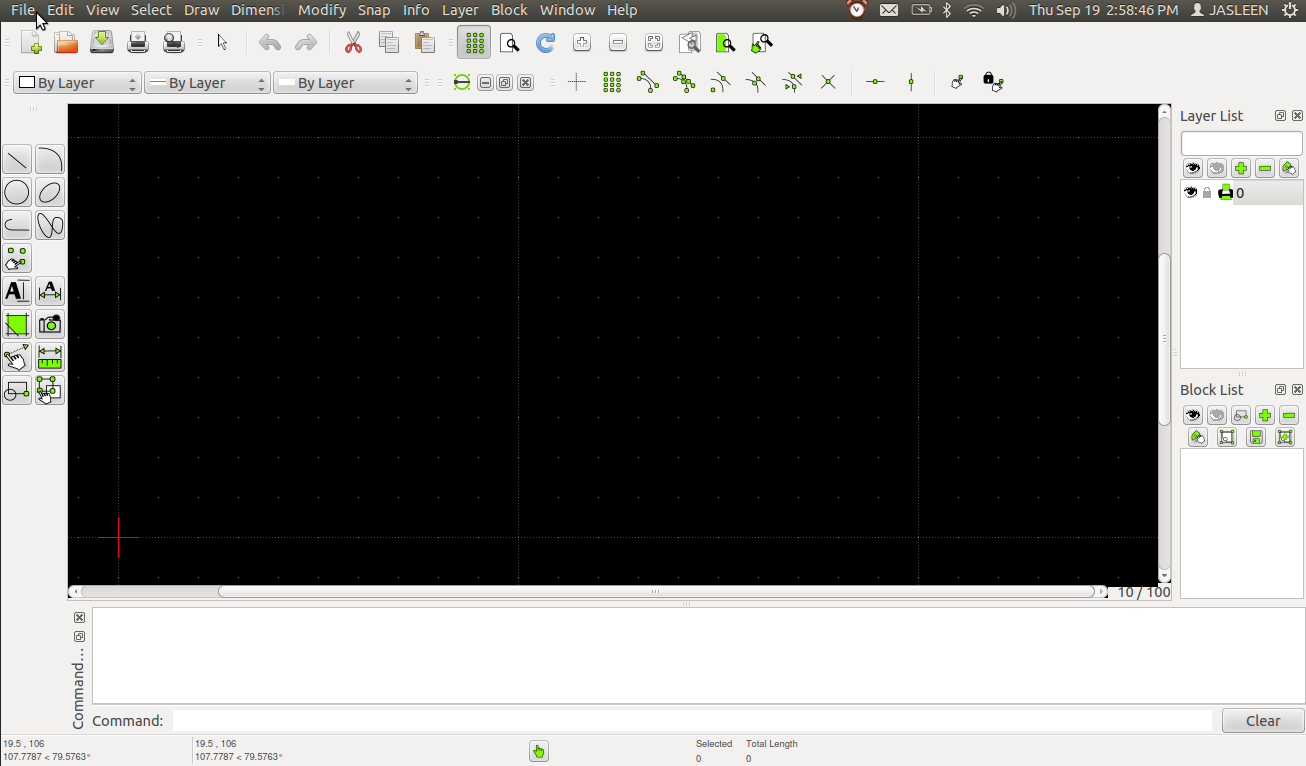
\includegraphics[width=450px]{./images/screen.png}
\caption{\small \sl User Interface of LibreCAD}
\end{figure}\\
%
\subsection*{LibreCAD window is divided into eight areas:}
\begin{enumerate}
\item{Menubar}
\item{Toolbar}
\item{Model Space}
\item{Layer Selection Box}
\item{Command Line}
\item{Status Line}
\item{Layer List}
\item{Block List}
\end{enumerate}
%
\begin{figure}[h!]
\centering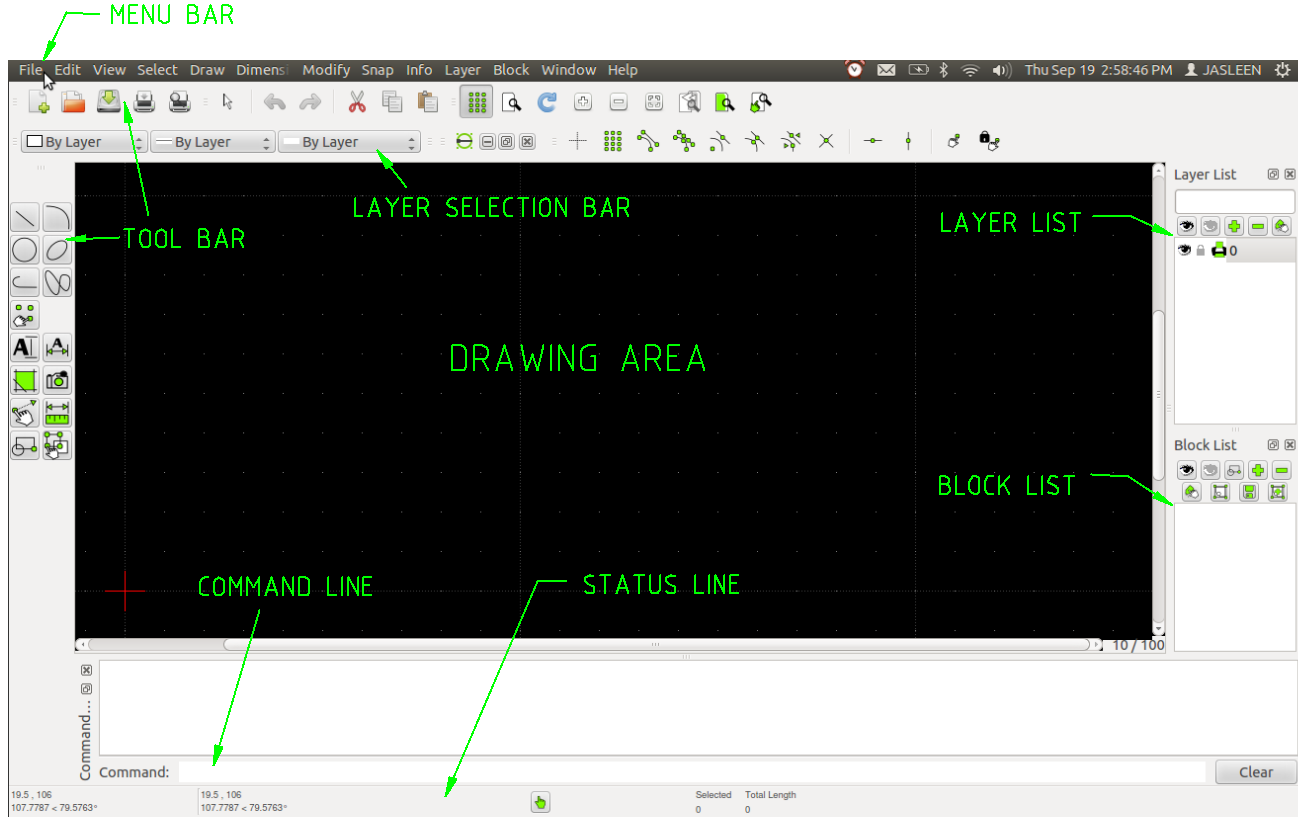
\includegraphics[width=450px]{./images/labelscreen.png}
\caption{\small \sl LibreCAD Screen}
\end{figure}
%
\textbf{\\\underline{Menu Bar:}}
A horizontal menu located on top that contains the major functions of CAD. When a function is selected from the menu, the menu drops down and displays further options under the menu. A number of options in the menu bar allows you to set program defaults and create a customized working environment.
\\\\
\textbf{\underline{Toolbar:}}
A collection of tool buttons grouped together. It is on the left side of the drawing window. Using tool bars is a very convenient method of entering commands, because you don't need to type on the keyboard or navigate through the menus. Each command is represented with a specific tool button in the tool bar. To enter a command, all you need to do is click on the tool button with the help of pointing device. It has nested toolbar in it. If you select circle, then it will display a varity of circles under a `circle' category. There is also a toolbar below the menu bar, which contains some common functions. LibreCAD allow you to customize the toolbars as needed. You can place
frequently used tool buttons in a tool bar, display only specific tool bars, and arrange them on the screen as you like.\\\\
\textbf{\underline{Model space/Drawing window:}}
The Drawing window or Model space is the area where you create your drawing. All the drawing work is confined within this area. The drawing
window may look small, but it has infinite size like the sky. You can draw as big or as small on this sky like drawing window. The view-display functions allow you to display specific views of the drawing.\\\\
\textbf{\underline{Layer Selection Box:}}
Layer Selection Box helps in selecting the Layer's atributes like: color, line type, thinkness.\\\\
\textbf{\underline{Command Line:}}
It is used to type commands. It notify you warnings or errors, if something is wrong. An area on the screen that shows all the commands being entered. You just need to remember the command names and type in command window to perform its function. Like, if you want to draw circle, then type `circle' in command window, it will ask you to enter the coordinates where to draw circle and with what radius.\\
Working with command window is fast and accurate method to draw. But you have to remember the command names to perform its function. These commands also has short commands, like to draw line, you can type 'line', 'ln' or 'l'\\\\
\textbf{\underline{Status Line:}}
The bottom bar of your screen which shows status of LibreCAD. Shows settings associated with the current drawing on the screen. It shows absolute and relative position of your mouse in cartesian and in polar coordinates. The mouse widgets shows the status of mouse left and right button. The `Selected Entities' shows you number of entities you selected. To enable/disable status bar, goto menu:  view $>$ status bar.\\\\
\textbf{\underline{Layer/ Block List:}}
It is on the right side of the drawing window. It shows the Layers and Blocks of currently opened Drawing.\\
\textbf{Layers} are used to keep same type of attributes in one layer. we can toggle the layers i.e to change the layers visible to hidden or vice-versa.\\
\textbf{Blocks} are used to use the block of a drawing, many times in our drawing.\\\\
%
\subsection*{\underline{Ways to communicate with LibreCAD:}}
\begin{itemize}
\item{Using the Menu Bar.}
\item{Using the tool bars.}
\item{Entering commands in the command window.}
\item{Working in the drawing area.}
\end{itemize}
%
\subsection*{\underline{Checking Version of LibreCAD:}}
It is important to check version of LibreCAD before starting work. LibreCAD version shoud be $>$=v2.0.*
If you have LibreCAD version less than this, then kindly switch to latest version as, the old version contains some bugs.
To check the version of your Application. Goto Help menu $>$ Select About. Ensure here the version of LibreCAD you using.\\\\
\begin{figure}[h!]
       \centering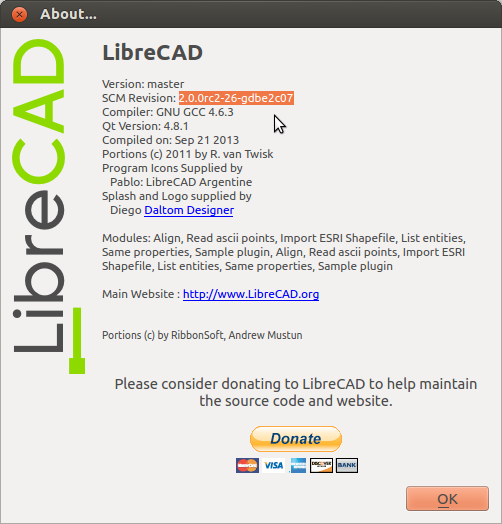
\includegraphics[width=230px]{./images/about.png}
       \caption{\small \sl About LibreCAD}
       \end{figure}

%
\newpage
\section{Preparing for Drawing}
\vspace{0.2in}  %to enter vertical space
\begin{enumerate}
\item{\textbf{\underline{Setting the units:}}
You can set the units for your drawing from Edit Menu.
    \begin{figure}[h!]
    \centering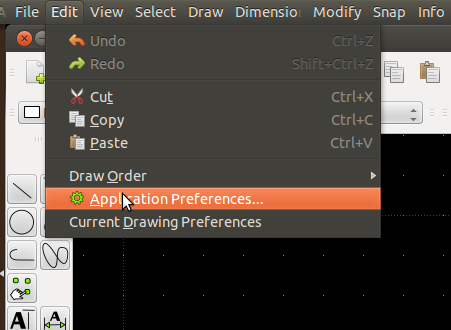
\includegraphics[width=200px]{./images/edit.png}
    \caption{\small \sl Edit menu}
    \end{figure}\\
You can either set your changes as a whole or for a current drawing.
If you make changes in \textbf{Application Preferences}, then these changes will reflect to your whole application.
And If you make changes in \textbf{Current Application Prefences}, then the changes reflect to your current Drawing only.\\\\
To set changes in your Current Drawing:
    \begin{enumerate}
    \item{Click on the \textbf{Edit} Menu}
    \item{then click on \textbf{Current Drawing Preferences}}
       \begin{figure}[h!]
       \centering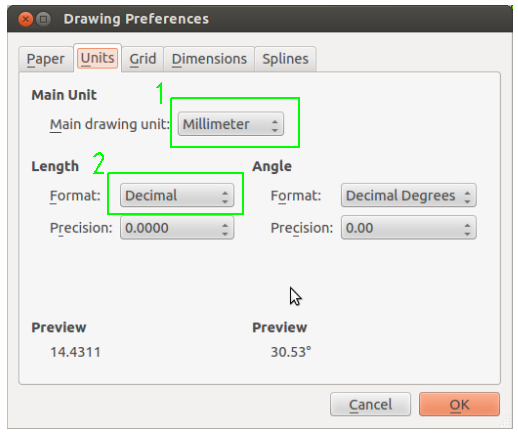
\includegraphics[width=200px]{./images/draw_pref.png}
       \caption{\small \sl Current Drawing Preference}
       \end{figure}
    \item{Goto \textbf{Units} tab,The units command allows setting the type of measurement and orientation of angular measurement.}
    \item{Select the \textbf{Main Drawing unit}. By default, it is set to Millimeter.}
    \item{Set the Format. There are different formats: Architectural, Decimal, Engineering, Fractional, Scientific.}
       \begin{figure}[h!]
       \centering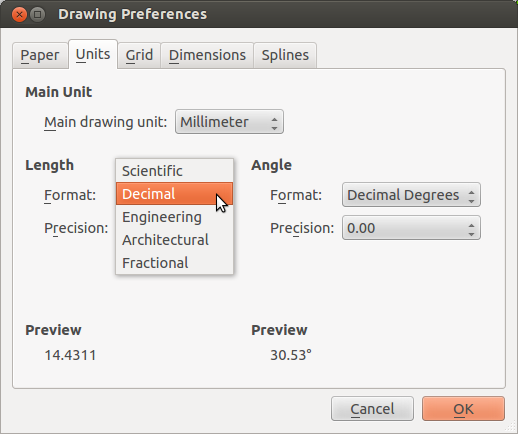
\includegraphics[width=200px]{./images/unitFormat.png}
       \caption{\small \sl Setting the Format for Length.}
       \end{figure}
    \end{enumerate}
}
\vspace{0.2in}
\item{\underline{\textbf{Snap and grid mode:}} Grid and Snap mode are used to learn, to restrict the movement of the cursor to a set increment on the screen. The GRID and SNAP MODE options can be turned ON or OFF from the icons or menubar or command line.\\
\textbf{Snap} feature allows you to precisely select grid points or significant points on existing objects: endpoints or midpoints of lines, etc. You can select snap option under 'Snap' Menu or from icons or from command line. Below is this image of icons of different type of snapping.
\vspace{.2in}
\begin{figure}[h!]
\begin{minipage}{.5\textwidth}
\centering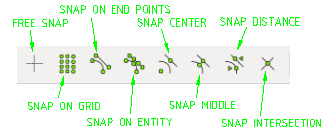
\includegraphics[width=210px]{./images/snap.png}
\caption{\small \sl Icons for Snapping}
\end{minipage}
\begin{minipage}{.5\textwidth}
       \centering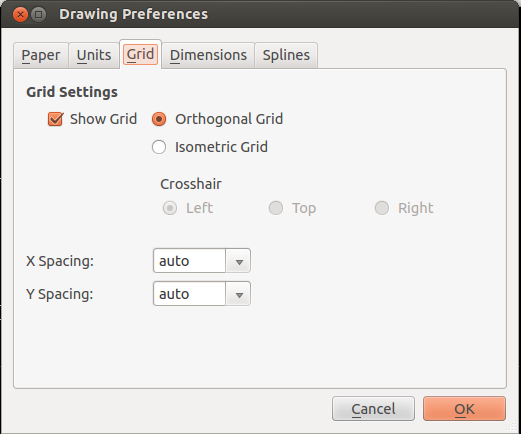
\includegraphics[width=180px]{./images/gridSet.png}
       \caption{\small \sl Choosing the type of Grid.}
       \end{minipage}
       \end{figure}}
\newpage
The \textbf{Grid\centering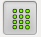
\includegraphics[width=20px]{./images/grid.png}}: A grid usually refers to two or more infinite sets of evenly-spaced parallel lines at particular angles to each other in a plane, or the intersections of such lines. It helps you align objects and visualize the distance between them. You can also change the color of Grid from Edit menu $>$ Application Prefences $>$ Grid color.\\
There are two types of grid: \textbf{orthogonal grids}, with two sets of lines perpendicular to each other (such as the square grid), and \textbf{isometric grids}, with three sets of lines at 60-degree angles to each other (such as the triangular grid). Isometric grid is used to depict 3D objects on a 2D surface.You can select type of Grid you want from Edit menu $>$ Current Drawing Preferences.
\vspace{0.2in}
\item{\textbf{\underline{\\Zooming and panning:}} Pan and zoom are very useful tools in LibreCAD. We can use Zoom or Pan command to navigate in our drawing.
\begin{figure}[h!]
\centering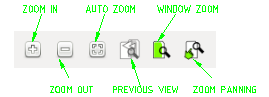
\includegraphics[width=240px]{./images/zoomPan.png}
\caption{\small \sl Icons for Zooming and Panning}
\end{figure}
\textbf{\\Zoom:} This tool increases / decreases the current viewing factor. The zoom tool is valuable when
you need to move up close to an entity to work on it. This is especially true when the
area is very small, or several lines drawn close together. As you will see in a moment,
there are several ways to use zoom: Zoom In, Zoom out, Auto Zoom, Window Zoom, Zoom panning.\\
\textbf{Panning:} Panning means moving around the drawing. Selecting the panning option you can drag your drawing. Pan allows you to dragging the drawing up, down, right, or left. This is especially useful if your drawing is large.}
\vspace{0.2in}
\item{\textbf{\underline{Dimentioning:}} To make changes in your application, goto `Application prefernces' under `Edit' menu. If you want to make changes in current drawing only, then goto to \textbf{Edit} $>$ \textbf{Current Preference}. Then selects the \textbf{Dimensions} tab.   
       \begin{figure}[h!]
       \centering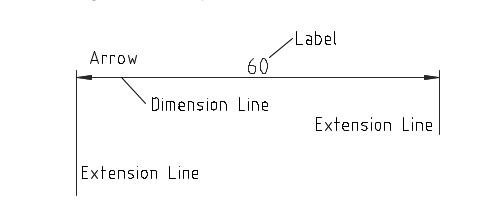
\includegraphics[width=230px]{./images/dimen.png}
       \caption{\small \sl Dimensioning}
       \end{figure}
       \begin{figure}[h!]
       \centering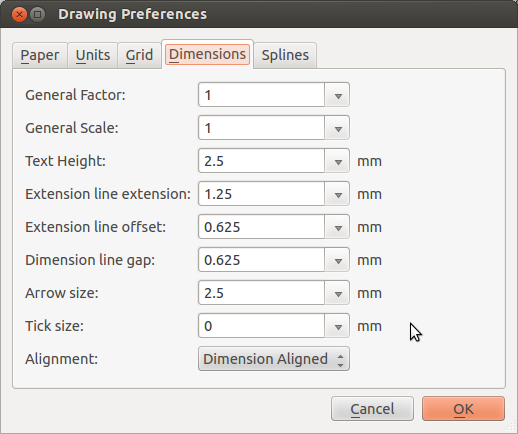
\includegraphics[width=200px]{./images/dimensions.png}
       \caption{\small \sl Setting Dimensioning for Drawing.}
       \end{figure}
}
%\vspace{0.2in}
\item{\underline{\textbf{\\\\Layers:}} Every entity of a drawing is on exactly one layer and a layer can contain
lots of entities. Typically entities with a common 'function' or common attributes are
put on the same layer. Layers are especially important in Assembly drawings. An Assembly drawing is a
drawing showing 2 or more parts as an assembly on a drawing. Each part is drawn on
its own layer and when all the layers are shown on the drawing you have the complete
assembly in view. You can create/ delete as much layers as you want, but their must be atlest one layer in drawing. By default there is one layer created, named `\textbf{0}'. Layers can have attributes (color, line width, line
style). Each entity can have its own attributes or have its attributes defined by the
layer it is placed on.
\begin{figure}[h!]
       \centering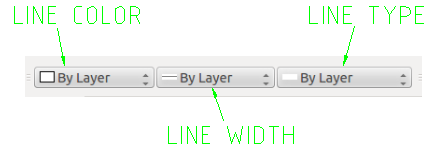
\includegraphics[width=230px]{./images/layer_set.png}
       \caption{\small \sl Icons for Layer}
       \end{figure}
     \begin{itemize}
     \item{\textbf{Line color:} You can select the color for your layer. This color will be same for all entities on a current Layer.}
     \item{\textbf{Line width:} You can select the width of line you want to use for your current layer.}
     \item{\textbf{Line type:} It provides you different types of lines: Dot, Dashed, Continous, Divid, Center, Border, No pen, etc.}
     \end{itemize}}
\end{enumerate}

%
\newpage
\section{Using Command Line} \vspace{.1in}
\textbf{\\DRAW Command}
\begin{table}[h!]\centering\begin{tabular}{|c|c|}
\hline Point & po, point\\
\hline Line & l, li, line\\
\hline Polyline & polyline\\
\hline LineParallel & o, offset, par, parallel\\
\hline Arc3P & a, arc\\
\hline Circle & ci, circle\\
\hline LineRectangle & rec, rectang, rectangle\\
\hline Text & text\\
\hline \end{tabular}\end{table} \vspace{.1in}
%
\textbf{\\ZOOM Command}
\begin{table}[h!]\centering\begin{tabular}{|c|c|}
\hline ZoomRedraw & zr, rg, regen, zoom - redraw\\
\hline ZoomWindow & zw, zoom - window\\
\hline ZoomAuto & za, zoom - auto\\
\hline ZoomPan & zp, zoom - pan\\
\hline ZoomPrevious & zv, zoom - previous\\
\hline \end{tabular}\end{table} \vspace{.1in}
%
\textbf{\\EDIT Command}
\begin{table}[h!]\centering\begin{tabular}{|c|c|}
\hline EditUndo & u, undo\\
\hline EditRedo & r, redo\\
\hline EditKillAllActions & k, kill\\
\hline \end{tabular}\end{table}\vspace{.1in}
%
\textbf{\\MODIFY Command}
\begin{table}[h!]\centering\begin{tabular}{|c|c|}
\hline ModifyTrim & xt, rm, modify - trim (extend)\\
\hline ModifyTrim2 & tm, modify - multi trim (extend)\\
\hline ModifyMove & mv, modify - move\\
\hline ModifyBevel & ch, modify - bevel (chamfer)\\
\hline ModifyMirror & mi, modify - mirror\\
\hline ModifyRotate & ro, modify - rotate\\
\hline ModifyScale & sz, modify - scale \\
\hline ModifyStretch & ss, modify - stretch\\
\hline ModifyDelete & er, modify - delete (erase)\\
\hline EditUndo & oo, modify - undo (oops)\\
\hline EditRedo & uu, modify - redo\\
\hline BlocksExplode & xp, modify - explode\\
\hline \end{tabular}\end{table} \vspace{.1in}
%
\textbf{\\TOOL Command}
\begin{table}[h!]\centering\begin{tabular}{|c|c|}
\hline ToolRegenerateDimensions & dimregen\\
\hline \end{tabular}\end{table} \vspace{.1in}
%
\textbf{\\DIMENSION Command}
\begin{table}[h!]\centering\begin{tabular}{|c|c|}
\hline DimAligned & da, dimension - aligned\\
\hline DimLinear & dr, dimension - linear\\
\hline DimLinearHor & dh, dimension - horizontal\\
\hline DimLinearVer & dv, dimension - vertical\\
\hline DimLeader & ld, dimension - leader\\
\hline \end{tabular}\end{table} \vspace{.1in}
%
\textbf{\\SNAP Command}
\begin{table}[h!]\centering\begin{tabular}{|c|c|}
\hline SnapFree & os, snap - none\\
\hline SnapGrid & sg, snap - grid\\
\hline SnapEndpoint & se, snap - end\\
\hline SnapIntersection & si, snap - intersection\\
\hline SnapCenter & sn, snap - center\\
\hline SnapMiddle & sm, snap - middle\\
\hline SnapOnEntity & np, snap - nearest point\\
\hline \end{tabular}\end{table} \vspace{.1in}
%
\textbf{\\SELECTION Command}
\begin{table}[h!]\centering\begin{tabular}{|c|c|}
\hline DeselectAll & tn, deselect - all\\
\hline \end{tabular}\end{table}\\[-1ex]
%

%
\newpage
\section{Play with LibreCAD} 
\vspace{.3in}  %to enter vertical space
\subsection*{Draw some basic}
\begin{enumerate}
\vspace{.25in}
\item{\textbf{Draw a Point:}
      \begin{enumerate}
      \item{Goto to toolbar, click on \textbf{Point} icon 
\includegraphics[width=20px]{./images/point.png}}
      \item{Click on Drawing area where you want to create point.}
      \end{enumerate}}
%
\vspace{.25in}
\item{\textbf{Draw a Line:}
      \begin{enumerate}
      \item{Goto to toolbar, click on \textbf{Line} icon 
\includegraphics[width=20px]{./images/line.png}}
      \item{A nested toolbar opens, which show you different functions for creating a line. Choose the \textbf{Line with two points }
\includegraphics[width=20px]{./images/line2p.png}}
      \item{Select first point on drawing area}
      \item{Select second point on Drawing area}  
      \end{enumerate}}
%
\vspace{.25in}
\item{\textbf{Draw a Arc}
    \begin{enumerate}
    \item{Goto to toolbar, click on \textbf{Arc} icon
\includegraphics[width=20px]{./images/arc.png}}
    \item{A nested toolbar opens, which show you different functions for creating an arc. Choose the \textbf{Arc with center, point, Angles }
\includegraphics[width=20px]{./images/arc_cpa.png}}
    \item{Specify a point on Drawing area as a center of an arc. Hold the left click and move your cursor. You will see a preciew of circle as you move your cursor. Left click to unhold the cursor.}
    \item{Select two points: first point as your Starting point of Arc and second point as your End point of Arc.} 
    \end{enumerate}}
%
\vspace{.25in}    
\item{\textbf{Draw a Circle}\begin{enumerate}
    \item{Goto to toolbar, click on \textbf{Circle} icon
\includegraphics[width=20px]{./images/circle.png}}
    \item{A nested toolbar opens, which show you different functions for creating an Circle. Choose the \textbf{Circle with center, point }
\includegraphics[width=20px]{./images/circle_cp.png}}
    \item{Specify a point on Drawing area as a center of an arc. Hold the left click and move your cursor. You will see a preciew of circle as you move your cursor. Left click to unhold the cursor.}\end{enumerate}}
%
\vspace{.25in}
\item{\textbf{Draw a Ellipses}\begin{enumerate}
    \item{Goto to toolbar, click on \textbf{Ellipses} icon
\includegraphics[width=20px]{./images/ellipse.png}}
    \item{A nested toolbar opens, which show you different functions for creating an Ellipses. Choose the \textbf{Ellipse with center and 2 points }
\includegraphics[width=20px]{./images/ellipse_c2p.png}}
    \item{Specify a point on Drawing area as a center of an arc. Hold the left click and move your cursor. You will see a preciew of ellipse as you move your cursor. Left click to unhold the cursor.}\end{enumerate}}
%
\vspace{.25in}
\item{\textbf{Draw a Polyline}
    \begin{enumerate}
    \item{Goto to toolbar, click on \textbf{Polyline} icon 
\includegraphics[width=20px]{./images/polyline.png}}
    \item{A nested toolbar opens, which show you different functions for creating an Polyline. Choose the \textbf{Create Polyline}
\includegraphics[width=20px]{./images/create_polyline.png}}
    \item{Click on one point on drawin are and then second point and then third...and so on till you want. To come out of this command, use Right click}
    \end{enumerate}}
%
\vspace{.25in}
\item{\textbf{Draw a Spline}\begin{enumerate}
    \item{Goto to toolbar, click on \textbf{Spline} icon 
\includegraphics[width=20px]{./images/spline.png}}
    \item{Define the points to which Spline go through. To come out of this command, use Right click}\end{enumerate}}
%
\vspace{.25in}
\item{\textbf{Draw a Text}\begin{enumerate}
    \item{Goto to toolbar, click on \textbf{Text} icon 
\includegraphics[width=20px]{./images/text.png}}
    \item{A dialog box will appear. Write the text you want on Dialog box and Set your text's font size and style. Then click on OK button
    \begin{figure}[h!] \centering 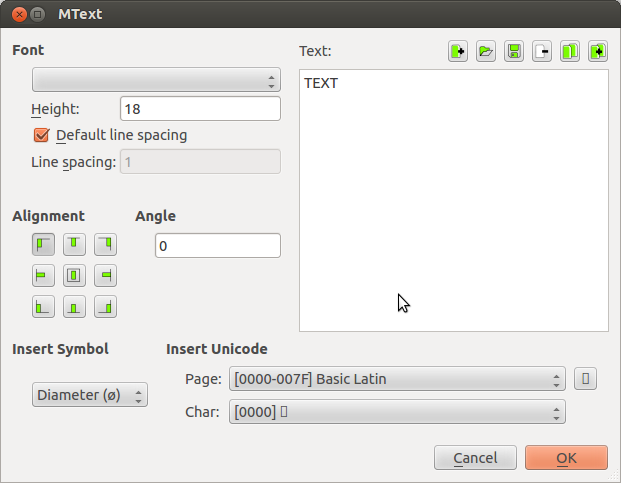
\includegraphics[width=200px]{./images/text_set.png} \end{figure}}
    \item{Specify the point on Drawing Area where you want to place your Text.}
    \end{enumerate}}
%
\vspace{.25in}
\item{\textbf{Draw a Image}\begin{enumerate}
    \item{Goto to toolbar, click on \textbf{Image} icon 
\includegraphics[width=20px]{./images/image.png}}
    \item{Select a image you want by browsing the images from your system}
    \item{select the point on drawing area where you want to place your image.}\end{enumerate}}
    %
\vspace{.25in}
\item{\textbf{Draw a Hatch}\begin{enumerate}
    \item{Goto to toolbar, click on \textbf{Text} icon 
\includegraphics[width=20px]{./images/hatch.png}}
    \item{Select the closed entity which you want to hatch.}
    \item{ click on run button 
\includegraphics[height=20px]{./images/run.png}}
    \item{A dialog box will be opened, select the type of hatch and set the angle, and then click OK button.}
    \end{enumerate}}
\end{enumerate}

\newpage
\section{Lets Draw Something}
\vspace{5 mm}  %to enter vertical space
\subsection{Lets Create a Yard}
\vspace{2mm}
\subsubsection*{\underline{Preparing for drawing:}}
\begin{itemize}
\item{\textbf{Setting the Units:} Goto to Edit menu $>$ Current Drawing Preference, goto Tab \textbf{Unit} $>$ select \textbf{Inch} as main Drawing units. Also select \textbf{Archtectural} as a Format of unit.
       \begin{figure}[h!]
       \centering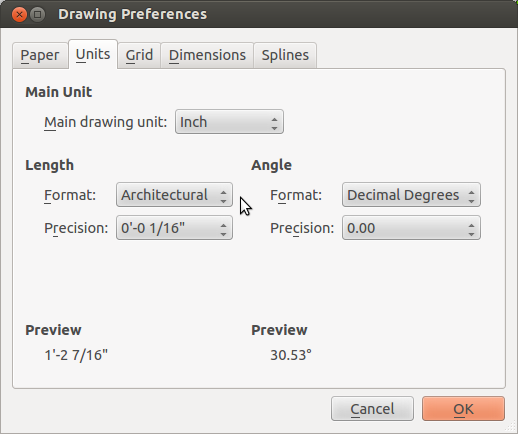
\includegraphics[width=220px]{./images-yard/units.png}
       \caption{\small \sl Setting Units for Yard}
       \end{figure}}
\item{\textbf{Turning ON Grid:} Goto to Edit menu $>$ Current Drawing Preference, goto Tab \textbf{Grid} $>$ check the \textbf{Show Grid} Option $>$ select \textbf{Orthogonal Grid}.
       \begin{figure}[h!]
       \centering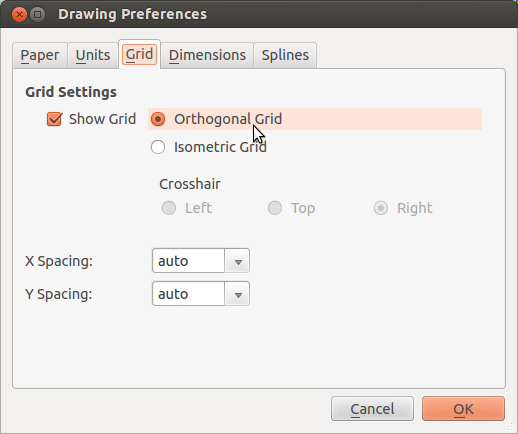
\includegraphics[width=220px]{./images-yard/grid.png}
       \caption{\small \sl Setting Grid for Yard}
       \end{figure}}
\item{\textbf{Turning ON Snap:} Goto Snap menu $>$ select \textbf{Snap on Grdi} for an instance. Snapping will be choosen to find accurate position according to the situation.
\begin{figure}[h!]
       \centering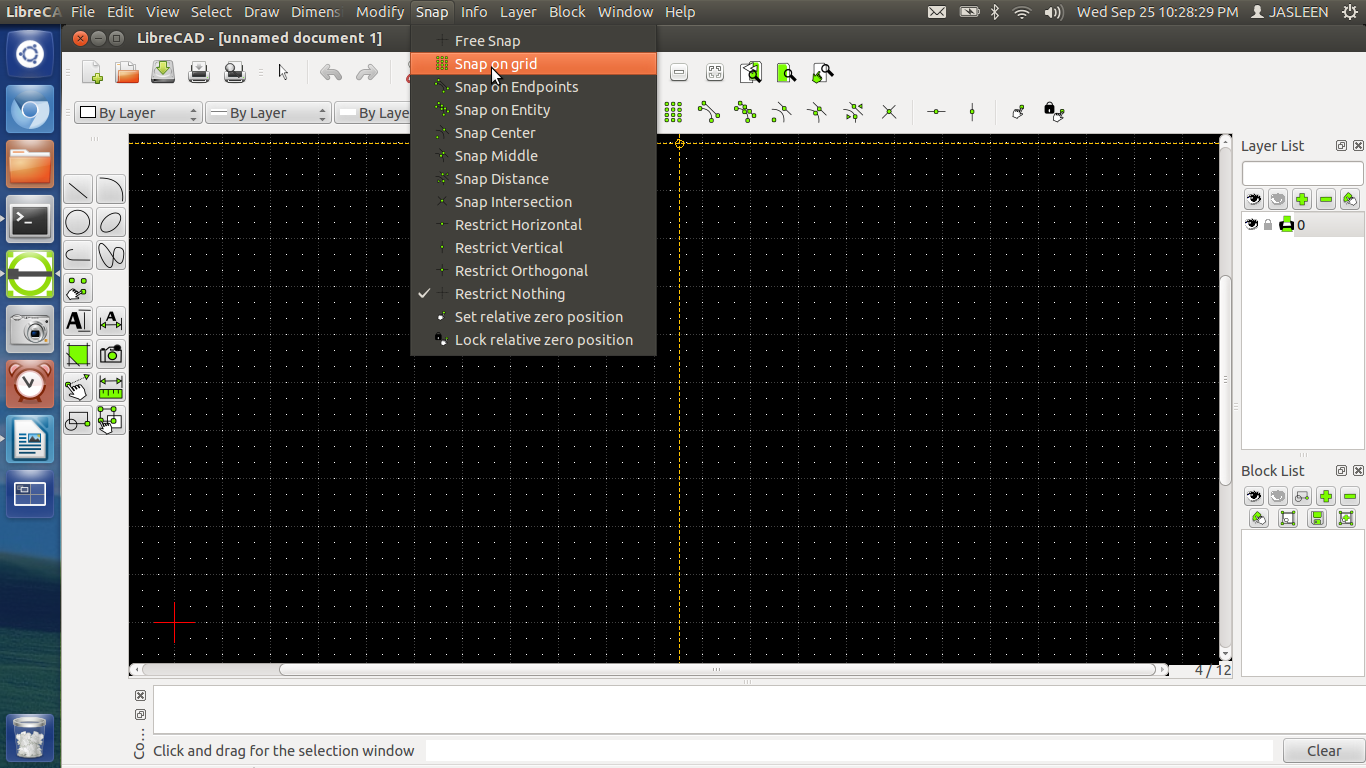
\includegraphics[width=400px]{./images-yard/snap.png}
       \caption{\small \sl Setting Grid for Yard}
       \end{figure}}
\end{itemize}\vspace{5mm}
%
\subsubsection*{\underline{Creating Layers:}}
On the Right side of screen, there is a \textbf{Layer List}, which is used to add/edit layers. Create a new Layer with $+$ icon. Add name of Layer and select its attributes.
\\Create these layers for Yard Drawing with following Colors and LineType.
       \begin{figure}[h!]
       \centering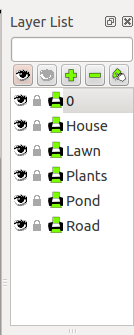
\includegraphics[width=60px]{./images-yard/layers.png}
       \caption{\small \sl Creating Layers}
       \end{figure}
\begin{table}[h!]\centering\begin{tabular}{|c|c|c|}
\hline \textbf{Name} & \textbf{Color} & \textbf{Line Type}\\ 
\hline House & White & Continous\\
\hline Lawn & Magenta & Continous\\
\hline Lot & Blue & Dash\\
\hline Plant & Green & Continous\\
\hline Pond & Cyan & Continous\\
\hline Road & Red & Continous\\
\hline Dimension & others(pink) & Continous\\
\hline \end{tabular}\end{table} 
\vspace{.3in}
%
\subsubsection*{\underline{Save the Drawing:}}
Now you can save your Drawing. Goto \textbf{File} menu $>$ \textbf{Save as.}
%
\newpage
\vspace{3mm}
\subsection*{\underline{Start Creating Drawing:}}\vspace{.5in}
\begin{enumerate}
\item{Make the \textbf{Lot} Layer active to Drawing Area, from Layer List.}
\item{Start Drawing with Line. Type `li' (shorthand for line) in Command Line. It will promp you:
\begin{verbatim}
Specify First point: 40,40
Specify next Point: @116<0
Specify next Point: @80<90
Specify next Point: @76<180
Specify next Point: @50<216.88
Specify next Point: @40,40
\end{verbatim}
Single \textbf{Right Click} is used to come out of \textbf{Line} Command. 
Here points are given as polar coordinates or cartesian coordinates\\
\textbf{(40,40)} is a cartesian coordinate, which (x,y) point with respect to absolute value(0,0).\\
\textbf{@116$<$0} is a polar coordinate, where, `@' is to use Relative cordinates, '116' is Distance in inch from previous end point, "$<$'is to draw angle, '0' is the degree of angle by line is drawn.\\\\
\begin{figure}[h!]
       \centering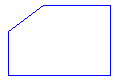
\includegraphics[width=180px]{./images-yard/lot.png}
       \caption{\small \sl Creating Lot of yard Drawing}
       \end{figure}
\\Now \textbf{Lot} is created, save your drawing as -  File $>$ Save.}
%
\item{Make the \textbf{House} Layer active to Drawing Area, from Layer List.}
\item{Select polyline entity by typing \textbf{polyline} in a Command Line.\\
Turn on \textbf{Snap on end point.}
\begin{verbatim}
Specify First point: <Pick lower Right corner of 'Lot' using snap on endpoint>
Specify next Point: @30<90
Specify next Point: @3<0
Specify next Point: @20<90
Specify next Point: @28<180
Specify next Point: @50<270
Specify next Point: <Pick lower Right corner of 'Lot' using snap on endpoint>
then right click to leave the polyline command.
\end{verbatim}
\begin{figure}[h!]
       \centering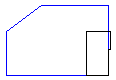
\includegraphics[width=180px]{./images-yard/house-rt.png}
       \caption{\small \sl Creating House of yard Drawing}
       \end{figure}
Use \textbf{Move} Command from \textbf{Modify} Menu, to move the House.
\begin{verbatim}
Specify to move: <Pick any point of house, whole house will be selected as one entity>
Specify Reference Point: <Pick any lower left corner of house>
Specify Target Point: @10<90
\end{verbatim} 
Again use Move Command.
\begin{verbatim}
Specify to move: <Pick any point of house, whole house will be selected as one entity>
Specify Reference Point: <Pick any lower left corner of house>
Specify Target Point: @20<-180
\end{verbatim} 
\begin{figure}[h!]
       \centering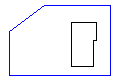
\includegraphics[width=180px]{./images-yard/house-mv.png}
       \caption{\small \sl Moving House to its position}
       \end{figure}
Now \textbf{House} is created, again save your drawing as -  File $>$ Save.}
%
\item{Make the \textbf{Road} Layer active}
\item{Select polyline.
\begin{verbatim}
Specify First point: <Pick upper Right corner of 'House' using Snap on Endpoint>
Specify next Point: @28<0
Specify next Point: @40<90
then right click to leave the polyline command.
\end{verbatim}
Select the Round Option from Modify menu, to round the turn of Road. Select the radius of round curve as 10.0 and also check the trim option to trim the intersecion of two lines.

\includegraphics[width=80px]{./images-yard/round.png}
\begin{figure}[h!]
       \centering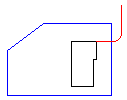
\includegraphics[width=160px]{./images-yard/round-c.png}
       \caption{\small \sl Creating one side of Road}
       \end{figure}
\\As one side of Road is created. Now create other side of road usinf Mirror command.
\\Turn ON snap on Entity, Middle, Distance.
\\Goto Modify $>$ Mirror.
\begin{verbatim}
Select the Entity: < select road>
Specify first point of Mirror Line:<pick a point vertical to house's left edge on right side>
Specify second point of Mirror Line:<pick a point vertical to house' left edge on left side>
\end{verbatim}
A mirror image appears in preview, set its angle by moving your cursor and then hit click to stay on that preview. A dialog box will open , select 'keep original'and then click OK.
\begin{figure}[h!]
       \centering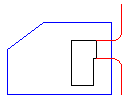
\includegraphics[width=160px]{./images-yard/road.png}
       \caption{\small \sl Creating other side of Road}
       \end{figure}
       Note: You can UNDO your mistake anytime.}
\item{Make the \textbf{Lawn} Layer active}
\item{Select Spline. Then select the middle of Lot (Diagonal side), using snap on Middle and Intersection. Click on middle point, then using Free snap, make a free-hand line with continuous clicks till it reach the other side of Lot.
\\Then selecting polyline and using Snap on Endpoint, cover the whole Lawn. Make sure to Lock all other Layers. So that you can easily pick point of your Lawn Layer. Locking a Layer is useful to select the objects overlaying on different layers. Locking makes the layer visible, but you cant pick that Locked Layer.
\begin{figure}[h!]
       \centering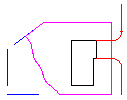
\includegraphics[width=180px]{./images-yard/lawn-full.png}
       \caption{\small \sl Lawn of Yard Drawing}
       \end{figure}
You can save your drawing now.}
\item{Make the \textbf{Plant} Layer active}
\item{Create a Block in a seperate drawing document and then import it in you drawing. Block is useful when we have to draw same thing at many places, with same/different scaling factor. Using Block we create the thing once, and used that block many times.\\
TO create a Block of Tree, First make a circle, and then a line crossing from its center (using Snap on Center) and coming smaller towards the outer of circle boundary. Now goto Modify menu $>$ Rotate. 
\begin{verbatim}
Select the Entity to rotate: <select line in circle>
Click on run.
Specify Rotation center: <select center of circle>
Specify Reference point: <select center of circle>
Specify Target point: <select center of circle>
\end{verbatim}
\vspace{.2in}
\begin{figure}[h!]
       \centering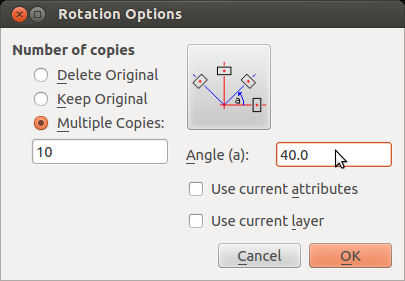
\includegraphics[width=210px]{./images-yard/rotate.png}
       \caption{\small \sl Rotate Dialogue box}
       \end{figure}
       \vspace{.5in}
       Set the rotate angle at 40 degree and keep multiple copies. A tree will be created.\\
Click on create Block option from Block menu. Select tree as whole entity to create a block.\\
click on run 
\includegraphics[width=40px]{./images-yard/run.png}\\
select reference point say (0,0)\\
Adialog box will appear, enter name of your Block (Tree). the click ok. A box will be created and will listed on Block List which is on right side below the layer List.\\
Goto Block menu $>$ Save your block as a seprate document. 
Now, you can insert this block wherever you want.
\\\\
To insert the block to your drawing. Open your drawing. Goto to File menu $>$ Import $>$ Block. Browse you block from your system. when you opened it, you will see the block appears in Block List.\\
Click on insert icon on Block List.\\
Specify any point as a reference point.\\
click on run.\\
insert the block where ever you want. you can scale your block by writting scale factor in box whick appears suring block command. or You can scale from Modify menu $>$ Scale.\\
Insert the tree block where you want on different scales.\\
\begin{figure}[h!]
       \centering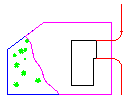
\includegraphics[width=180px]{./images-yard/tree.png}
       \caption{\small \sl Inserted Tree blocks in Plant Layer}
       \end{figure}}
\item{Make the \textbf{Dimension} Layer active. Create pond using Ellipse.}
\item{Make the \textbf{Fence} Layer active}
\item{Select Polyline to draw Fence. Here snapping will be trickly most used. 
\begin{verbatim}
Specify First point: <Pick middle 'House' using Snap on Middle and snap on Entity>
Specify next Point: <To select next point, Restrict vertical and on Entity>
Specify next Point: <Now unselect Restrict Veritcal and select snap on Endpoint>
Specify next Point: <select point using snap on Endpoint>
Specify next Point: <select point using snap on Endpoint>
Specify next Point: <select point using snap on Endpoint>
Specify next Point: <select point by selecting Restrict Orthogonaly, select the point by matching Crosshairs with the first line you created with same command>
Specify next Point: <select last point using snap on Entity>
then right click to leave the polyline command.
\end{verbatim}
\begin{figure}[h!]
       \centering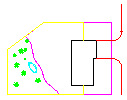
\includegraphics[width=180px]{./images-yard/fense.png}
       \caption{\small \sl Fense in yard}
       \end{figure}}    
\item{Make the \textbf{Dimension} Layer active\\
In Dimension Layer, we will add Text and Dimensions both at same layer.\\
To add Text, Goto Draw menu $>$ Text. A dialogue box will appear, Enter your text, select the Height of text and angle by which you rotate text. then click OK. Place your text in drawing area where you want.\\
To add Dimensions, goto Dimension Menu, select type of dimension. I used Vertical, Horizonal, alligned dimensions in my drawing and also Leder to indicate some part of Drawing.
\begin{figure}[h!]
       \centering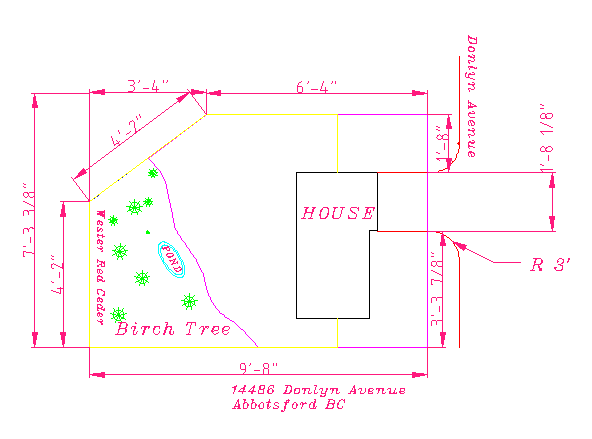
\includegraphics[width=380px]{./images-yard/dimension.png}
       \caption{\small \sl Drawing of Yard with Dimensioning}
       \end{figure}
\newpage
\large{The complete Drawing of Yard:}      
\begin{figure}[h!]
       \centering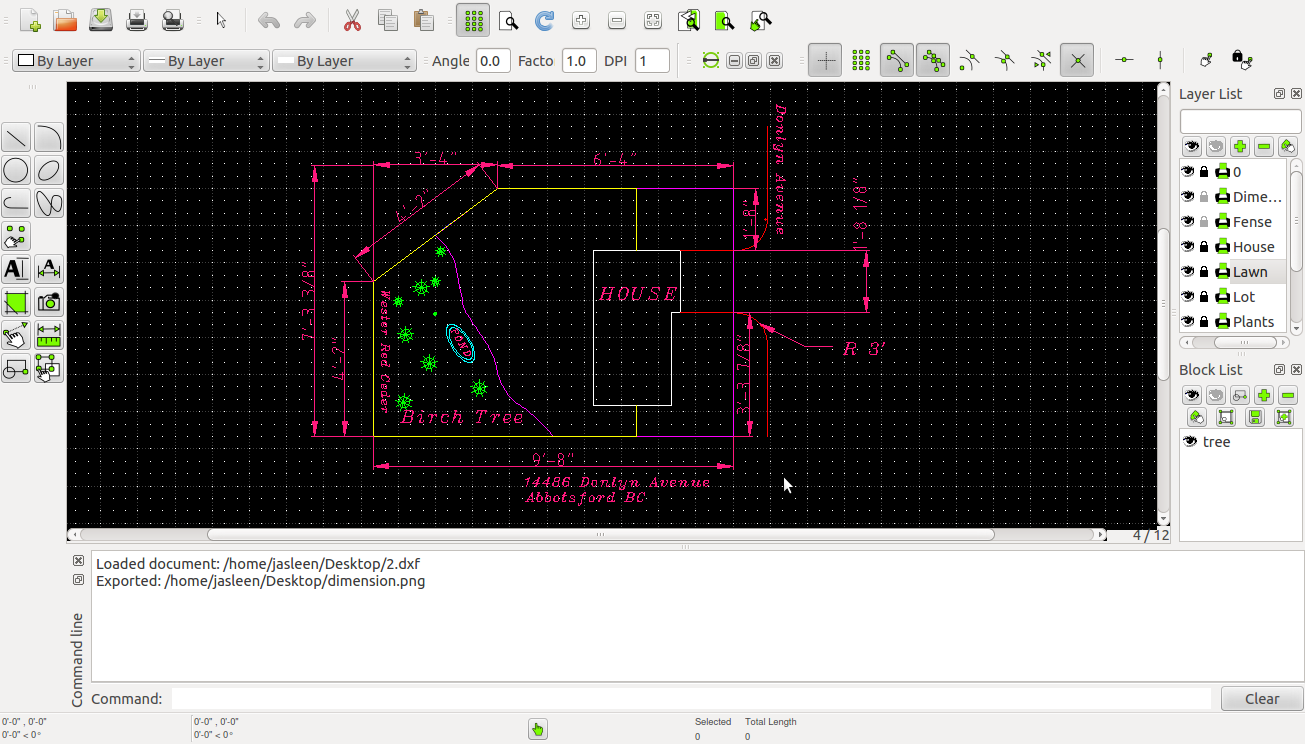
\includegraphics[width=450px]{./images-yard/complete.png}
       \caption{\small \sl Drawing of Yard with Dimensioning}
       \end{figure}}
\end{enumerate}

\newpage
    \begin{thebibliography}{5}
    \bibitem{vark:knud} http://librecad.org
    \bibitem{vark:knud} http://wiki.librecad.org
    \end{thebibliography}
\end{document}
